\chapter{Setup}

\section{Web Server}

A configuração do web server foi similar à do projecto anterior. Foi utilizado o \textbf{Apache} para dar host a um site nas porta 80 (default http) e 81.
Como isto já foi analisado no trabalho anterior. não será apresentada uma análise profunda da sua configuração \cite{apache}.

\section{FTP server}

A ferramenta selecionada para criar um servidor FTP foi o \textbf{Vsftpd}. Seguindo o guia de instalação \cite{vsftpd},
definimos um \textit{username} (testuser), com uma \textit{password}, que corresponde ao \textit{login} para aceder ao servidor.
O diretório predefinido num acesso FTP é \verb|\home\testuser|. 
Para efeitos de teste, colocamos nesse diretório um ficheiro \textit{test.txt}. 
De seguida, através do Firefox, onde já tínhamos o proxy configurado (Lab1), acedemos ao servidor
através do endereço \textit{ftp://172.16.1.12}, sendo que depois do login com as credenciais definidas, foi-nos possível aceder ao ficheiro.
Para fazer acessos FTP dos próprios \textit{tux}s, foi criado um script que ao ser executado,
faz download do ficheiro \textit{test.txt} presente no diretório:
\begin{lstlisting}
    #!/bin/sh
    HOST='172.16.1.12'
    USER='testuser'
    PASSWD='testuser'
    FILE='test'

    ftp -n $HOST <<END_SCRIPT
    quote USER $USER
    quote PASS $PASSWD
    get $file
    quit
    END_SCRIPT
    exit 0
\end{lstlisting}

\section{NTP Server}

O serviço requere duas componentes: um servidor e um cliente. O servidor NTP irá estar sincronizado com os servidores a nível internacional, e o cliente com o servidor NTP.
Durante a configuração do NTP server \cite{ntp}, definimos no ficheiro de configuração com 3 servidores internacionais para sincronização, indicados em 

\textit{https://support.ntp.org/bin/view/Servers/NTPPoolServers}.

Neste caso, os servidores indicados para a região de Portugal são:
\begin{itemize}
    \item server 1.pt.pool.ntp.org
    \item server 0.europe.pool.ntp.org
    \item server 1.europe.pool.ntp.org
\end{itemize}

No cliente, no ficheiro \verb|\etc\hosts| colocamos o IP do servidor NTP de modo a que o nome depois seja resolvido.
No ficheiro de configuração do NTP, adicionamos apenas o server \textit{NTP-server-host prefer iburst}.
A sincronização desta máquina será agora feita pelo servidor NTP.

Correr o comando \textit{ntpq -p} comprova o correto funcionamento do serviço (Fig \ref{fig:ntp_1}).

\begin{figure}
    \centering
    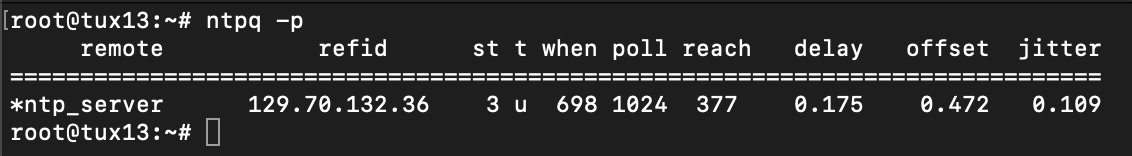
\includegraphics[width=.8\linewidth]{figs/setup/ntp_1.png}
    \caption{Servidor NTP do cliente}
    \label{fig:ntp_1}
\end{figure}


\section{Email Server}

Para criar um servidor email utilizamos o \textbf{Postfix}. Esta ferramenta é o MTA (Mail Transfer Agent) predefinido do Ubuntu e a sua instalação é simples \cite{postfix}.
Os endereços de mail gerados pelo Postfix são \textit{user@tux99.netlab.fe.up.pt}, onde o \textit{user} é "netlab" e o \textit{tux99} o "hostname" do computador.

Após a instalação do Postfix, fizemos um teste na porta 25 onde o serviço de email opera. Observamos a resposta do serviço ESMTP Postfix,
garantindo que a instalação tinha sido bem sucedida (Fig \ref{fig:webmail_1}).
\begin{figure}
    \centering
    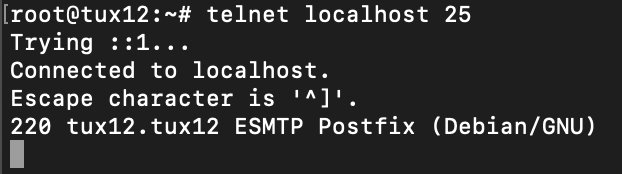
\includegraphics[width=.8\linewidth]{figs/setup/webmail_1.png}
    \caption{Teste telnet na porta 25}
    \label{fig:webmail_1}
\end{figure}

Para verificar o funcionamento do serviço, enviamos emails dentro da rede local para o \textit{tux13}, onde o Postfix também tinha sido configurado (Fig \ref{fig:webmail_2}).
Verificamos o ficheiro \verb|\var\log\mail.log| para ver se o email tinha sido enviado com sucesso.
De seguida fomos ao \textit{tux13}, onde no ficheiro \verb|\var\spool\mail\netedu| podemos ler o email que foi recebido ((Fig \ref{fig:webmail_3}).)
Desta modo, ficou garantido o funcionamento do servidor de email na rede local.

\begin{figure}
    \centering
    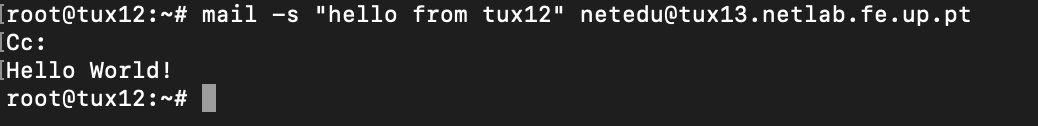
\includegraphics[width=.8\linewidth]{figs/setup/mail_2.png}
    \caption{Email enviado do tux12}
    \label{fig:webmail_2}
\end{figure}

\begin{figure}
    \centering
    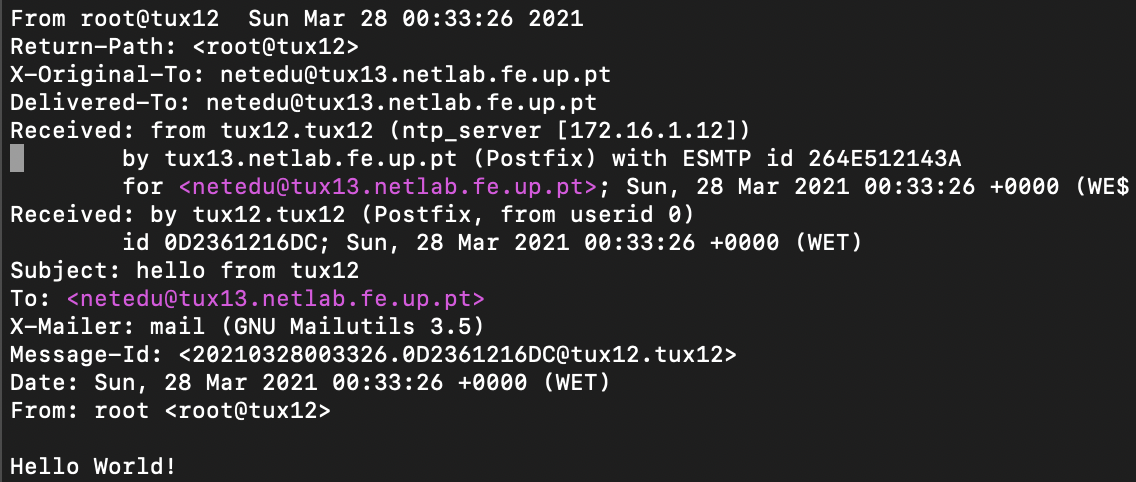
\includegraphics[width=.8\linewidth]{figs/setup/mail_3.png}
    \caption{Log do email recebido no tux13}
    \label{fig:webmail_3}
\end{figure}

\section{DNS Cache Server}

Um servidor DNS tem como função traduzir nomes em Ip's. A funcionalidade de cache permite que essa informação possa ser guardada localmente.
Desde modo, quando escrevemos um endereço, em vez de acedermos aos DNS servers do nosso ISP, temos essa informação guardada localmente, o que permite uma \textit{query} mais rápida.

O software utilizado foi o \textbf{Bind9}, predefinido do Ubuntu \cite{dns}.
Durante a configuração, foram adicionados os DNS servers do nosso ISP.
Procedemos à configuração quer da \textit{Forward Zone File} e do \textit{Reverse Zone File}.
Para testar o serviço, fez-se uso do comando \verb|dig @localhost google.com| (Fig \ref{fig:dns_1}).

\begin{figure}
    \centering
    \begin{subfigure}{.5\textwidth}
      \centering
      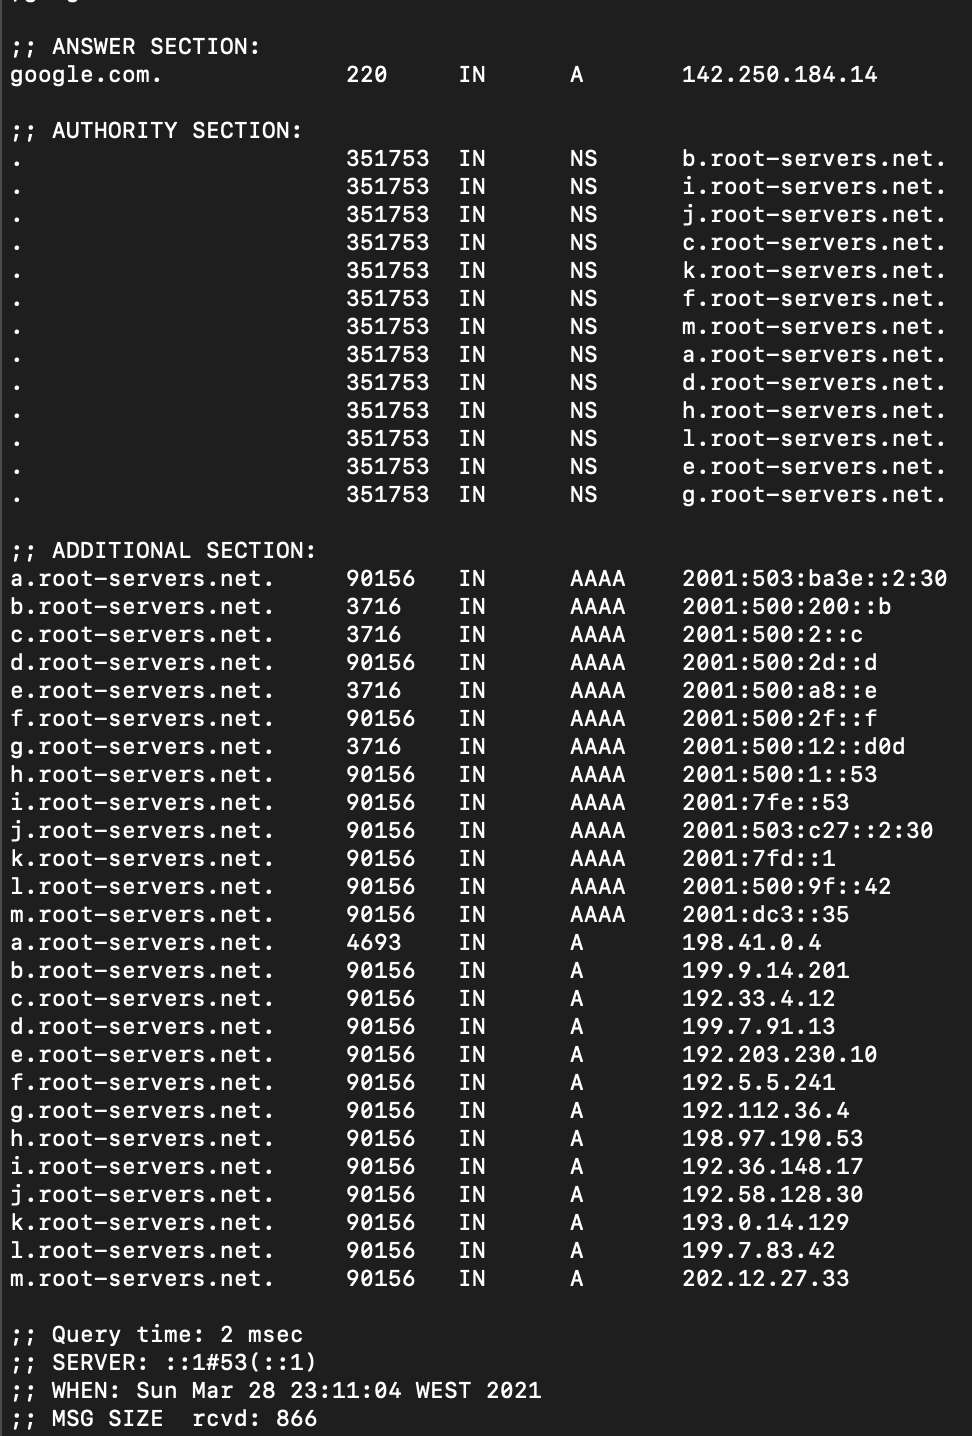
\includegraphics[width=.9\linewidth]{figs/setup/dns_1.png}
      \caption{Primeiro DNS query a google.com}
      \label{fig:dns_1}
    \end{subfigure}%
    \begin{subfigure}{.5\textwidth}
      \centering
      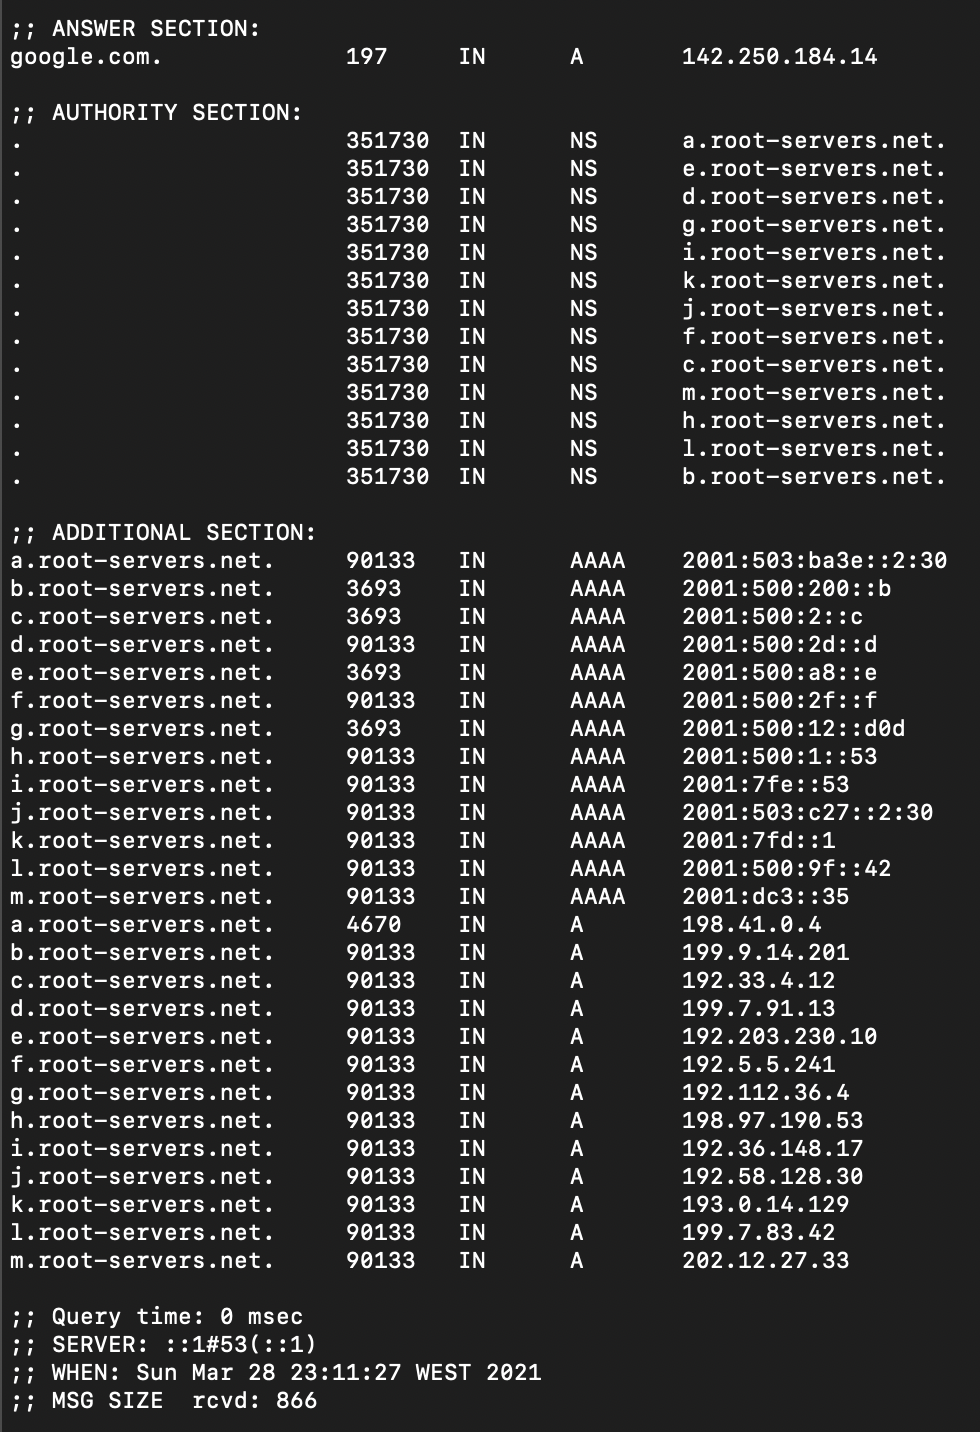
\includegraphics[width=.9\linewidth]{figs/setup/dns_2.png}
      \caption{Segunda DNS query a google.com}
      \label{fig:dns_2}
    \end{subfigure}
    \caption{Dns Queries}
    \label{fig:dns}
\end{figure}

Como se pode observar ao correr o comando a segunda vez, o query time é de 0 ms, dado que a informação ficou guardada em cache (Fig \ref{fig:dns_2}).
Passado um período de tempo predefinido no sistema, esta cache é limpa e um novo query é efetuado ao servidor DNS do ISP.





